\chapter{Analysis}
\label{ch:analysis}
\graphicspath{{Chapter-Analysis/figures/}}

\section{Data set}

The analyses presented in this thesis use the data from the \ac{LHC} 2013 \pPb at a center-of-mass energy of \pPbenergy with an integrated luminosity of \pPblumi.
The Pb ions had an energy per nucleon of 1.57 \TeV and collided with the 4 \TeV proton beam resulting in a net longitudinal boost of the center-of-mass system of $\ycm = 0.465$ in the proton direction relative to the ATLAS laboratory frame.
The \pPb\ run was divided into two periods between which the directions of the proton and lead beams were
reversed. 
The data are presented using the convention that the proton beam travels in the forward ($+z$) direction and the lead beam travels in the backward ($-z$) direction.
When the data from these two periods are combined, the \minbias triggers sampled a total luminosity, after prescale, of $24.5~\mu\textrm{b}^{-1}$ and yielded a total of 44 million events over the full centrality.

For results reported as a function of centrality, an additional \ac{HighET} trigger selection is included in the most central bin that requires the total transverse energy in both sides of the \ac{FCal} to be at least 65 \GeV.
The \ac{HighET} trigger sampled a total luminosity of $41.4~\mu\textrm{b}^{-1}$ after prescale and yielded 700 thousand events to the sample.
Events from this trigger are only included in the 0--1\% centrality interval, where the \ac{HighET} trigger is fully efficient.

The azimuthally-dependent results use central events with offline charged-particle multiplicity \Nch of at least 150, where only tracks with $\pt > 400~\MeV$ are counted in this number.
Several \acp{HMT} are included to boost the sample, with offline \Nch cutoffs at 100, 130, 150, 180, 200, and 225 tracks.
These \acp{HMT} provide a crucial 6.7 million events, as the \minbias triggers provide only 200 000 events at $\Nch > 150$.

All events are required to pass a set of \minbias selection criteria.
Events are required to be included in the latest Good Runs List from ATLAS, which rejects events recorded in conjunction with a technical difficulty in the detector.
The \minbias trigger requires either one hit in both sides of the \ac{MBTS} or two hits in one side.
Additional \ac{HighET} and high multiplicity triggers are included in some analysis bins as discussed above.
%% Events with an offline multiplicity lower than the nominal trigger threshold are excluded, as each of these HMTs reaches an efficiency near 1 near their nominal turn-on. This rejects events that fire a trigger in its turn-on region, as these samples can in principle be biased.
%% In practice no significant difference in the results is observed whether or not events in the HMT triggers' turn-ons are included, so using the nominal turn-on multiplicity is sufficient.
A timing cut is placed on the \ac{MBTS} hits in each side such that $|\Delta t_{AC}| < 10~\textrm{ns}$.
No more than one reconstructed \ac{PV} or strong vertex (where a strong vertex has more than 10 tracks or a total \pt of tracks greater than $6~\GeV$) is permitted in each event.
Diffractive events are identified for rejection by a gap of two units of pseudorapidity in event activity on the Pb-going side of the calorimeters \cite{HION-2012-15}.
Pileup events are also discarded using a run-dependent upper limit on the Pb-going \ac{ZDC}.
In addition, events are discarded if an error flag is recorded in the \ac{LAr} or tile calorimeter systems, or if there is an indication that the event was not completely recorded.

\section{Centrality determination}

\begin{figure}[t]
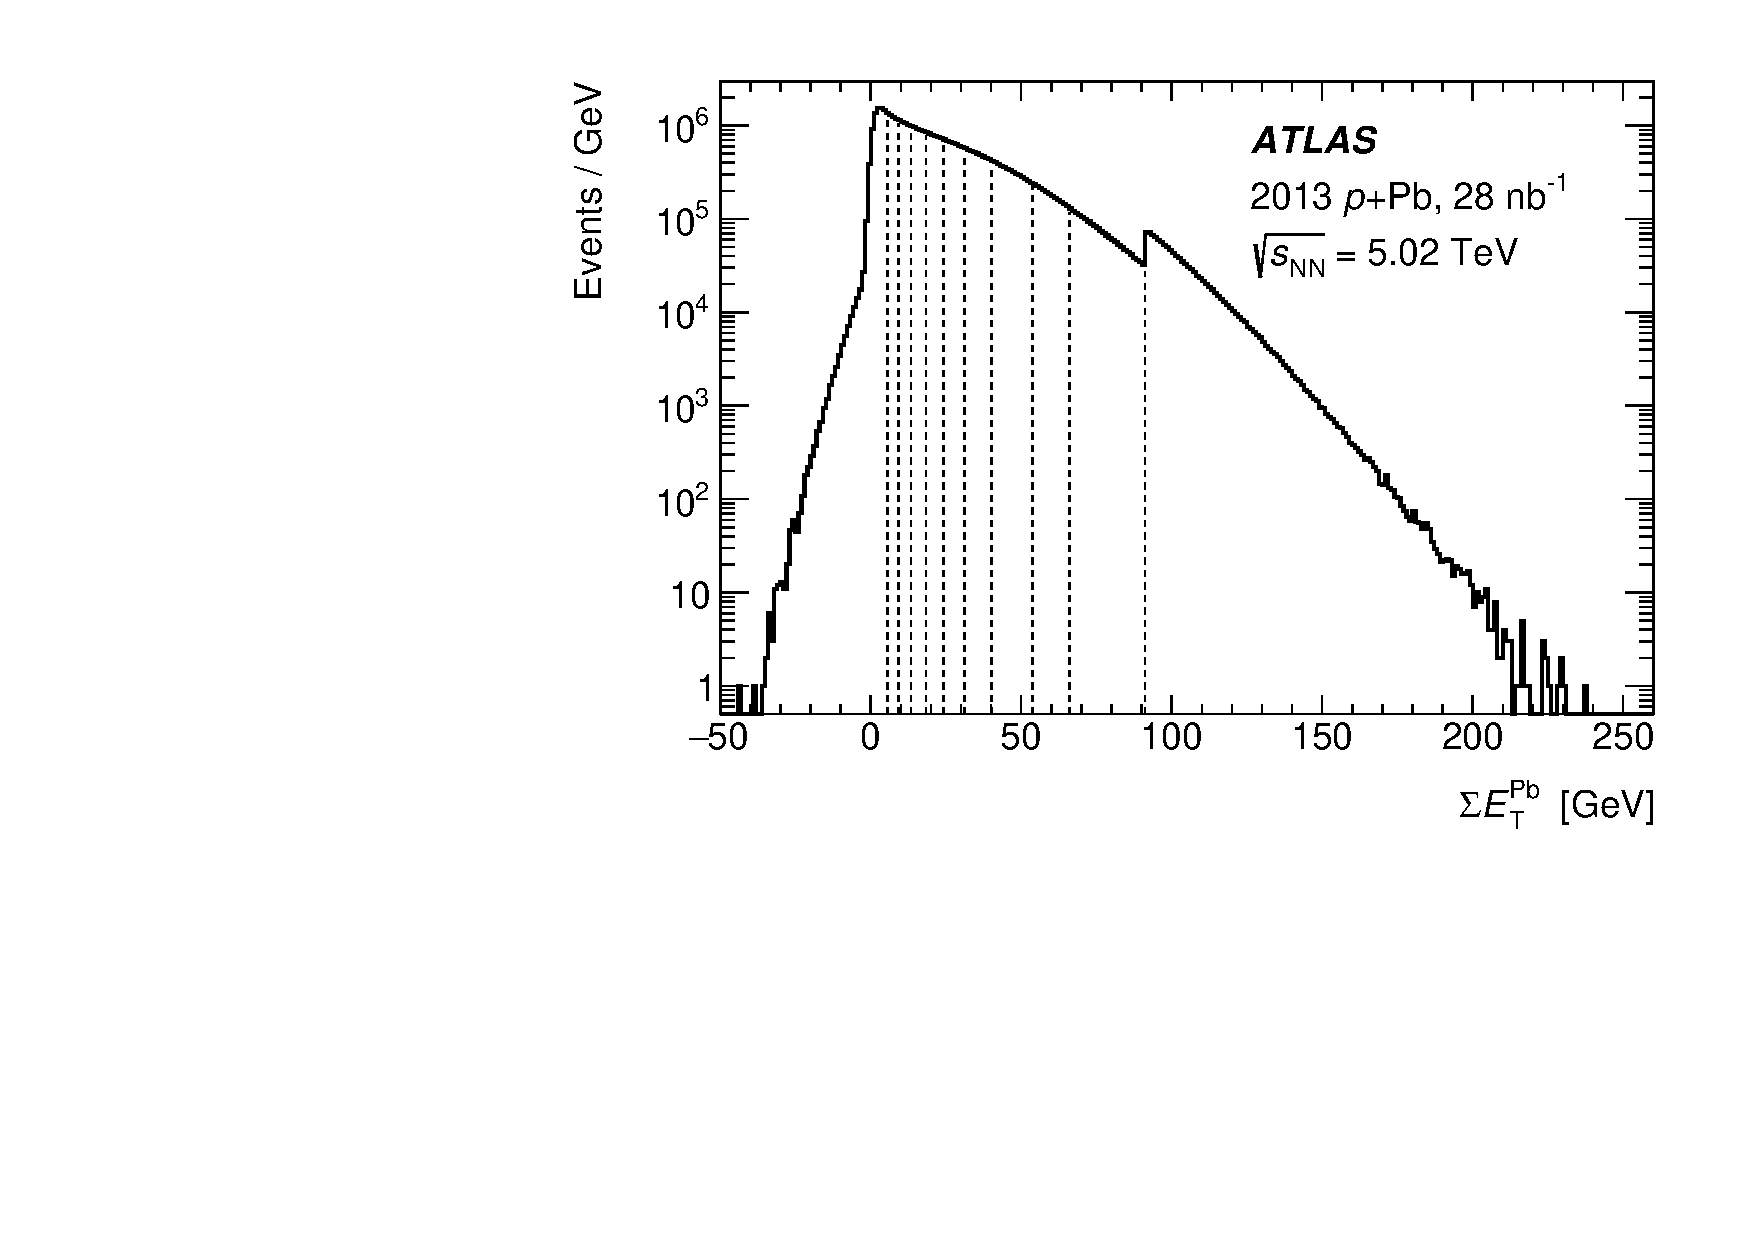
\includegraphics{fcal_et_total.pdf}
\caption{The distribution of the total transverse energy in the \ac{FCal} in the Pb-going direction (\sumETPb) for the events used in the centrality-dependent analysis. Dashed lines are shown at the boundaries of the centrality intervals, and the discontinuity at $\sumETPb = 91.08~\GeV$ corresponds to the lower \sumETPb boundary of the 0--1\% centrality interval.}
\label{fig:fcal_et}
\end{figure}

The centralities of the \pPb\ events are characterized following the procedures described in \Ref{\cite{HION-2012-15}}, using the total transverse energy in the Pb-going side of the \ac{FCal}, \sumETPb.
The use of the \ac{FCal} for measuring centrality has the advantage that it is not sensitive to multiplicity fluctuations in the kinematic region covered by the inner detector, where the measurements are performed.
Measurements are presented in this paper for the centrality intervals listed in \Cref{table:npart}.
The events selected using the \ac{HighET} trigger are used only in the 0--1\% centrality interval.
\Cref{fig:fcal_et} shows the distribution of \sumETPb\ values obtained from events included in this
measurement.
The discontinuity in the spectrum occurs at the low edge of the 0--1\% centrality interval, above which the \ac{HighET} events are included.

For each centrality interval, the average multiplicity of charged particles with $\pt > 100~\MeV$ and $|\eta| < 1.5$, \avgdNdeta, and the corresponding average number of participating nucleons, \avgNpart, are obtained from a previous publication \cite{HION-2012-15}.
Since this analysis uses finer centrality intervals (no wider than 10\% of the total centrality range) than
those used in \Ref{\cite{HION-2012-15}}, a linear interpolation over the Glauber \avgNpart is used to construct additional values for \avgdNdeta based on the published results.
This interpolation is justified by the result in \Ref{\cite{HION-2012-15}} that charged-particle multiplicity is proportional to \avgNpart in the peripheral region.
The values and uncertainties from this procedure are listed in \Cref{table:npart}.


\renewcommand{\arraystretch}{1.1}
\begin{table}
\begin{center}
\begin{tabular}{r || c | c | c || c}
\hline
 & \multicolumn{3}{c||}{\avgNpart} & \\ \cline{2-4}
Centrality & Glauber & GGCF $\omega_{\sigma} = 0.11$ & GGCF $\omega_{\sigma} = 0.2$ & $\avgdNdeta$\\
\hline \hline
0--1\% & $ 18.2^{+2.6}_{-1.0} $ & $ 24.2^{+1.5}_{-2.1} $ & $ 27.4^{+1.6}_{-4.5} $ & $58.1\ \pm 0.1\ \ \pm 1.9\ $ \\[2pt]
\hline
1--5\% & $ 16.10^{+1.66}_{-0.91} $ & $ 19.5^{+1.2}_{-1.3} $ & $ 21.4^{+1.5}_{-2.0} $ & $45.8\ \pm 0.1\ \ \pm 1.3\ $ \\[2pt]
\hline
5--10\% & $ 14.61^{+1.21}_{-0.82} $ & $ 16.5^{+1.0}_{-1.0} $ & $ 17.5^{+1.1}_{-1.1} $ & $38.5\ \pm 0.1\ \ \pm 1.1\ $ \\[2pt]
\hline
10--20\% & $ 13.05^{+0.82}_{-0.73} $ & $ 13.77^{+0.79}_{-0.81} $ & $ 14.11^{+0.86}_{-0.79} $ & $32.34 \pm 0.05 \pm 0.97$ \\[2pt]
\hline
20--30\% & $ 11.37^{+0.65}_{-0.63} $ & $ 11.23^{+0.62}_{-0.67} $ & $ 11.17^{+0.68}_{-0.62} $ & $26.74 \pm 0.04 \pm 0.80$ \\[2pt]
\hline
30--40\% & $ 9.81^{+0.56}_{-0.57} $ & $ 9.22^{+0.50}_{-0.54} $ & $ 8.97^{+0.60}_{-0.49} $ & $22.48 \pm 0.03 \pm 0.75$ \\[2pt]
\hline
40--50\% & $ 8.23^{+0.48}_{-0.55} $ & $ 7.46^{+0.41}_{-0.43} $ & $ 7.15^{+0.54}_{-0.39} $ & $18.79 \pm 0.02 \pm 0.69$ \\[2pt]
\hline
50--60\% & $ 6.64^{+0.41}_{-0.52} $ & $ 5.90^{+0.36}_{-0.34} $ & $ 5.60^{+0.47}_{-0.30} $ & $15.02 \pm 0.02 \pm 0.62$ \\[2pt]
\hline
60--70\% & $ 5.14^{+0.35}_{-0.43} $ & $ 4.56^{+0.32}_{-0.26} $ & $ 4.32^{+0.41}_{-0.23} $ & $11.45 \pm 0.01 \pm 0.56$ \\[2pt]
\hline
70--80\% & $ 3.90^{+0.24}_{-0.30} $ & $ 3.50^{+0.22}_{-0.18} $ & $ 3.34^{+0.29}_{-0.16} $ & $ \ \  8.49 \pm 0.02 \pm 0.51$ \\[2pt]
\hline
\end{tabular}
\caption{The average number of nucleon participants \avgNpart \cite{HION-2012-15} for each centrality interval in the Glauber model as well as the two choices for the Glauber-Gribov model with color fluctuations (GGCF) \cite{Alvioli:2013vk} (and references therein), along with the average multiplicity with $\pt > 100~\MeV$ and $|\eta| < 1.5$ also obtained from Ref.~\cite{HION-2012-15}. The parameter $\omega_{\sigma}$ represents the size of fluctuations in the nucleon-nucleon cross section. Asymmetric systematic uncertainties are shown for \avgNpart. The uncertainties in \avgdNdeta are given in the order of statistical followed by systematic.}
\label{table:npart}
\end{center}
\end{table}

 


\section{Flow vector determination}
%% \section{Correlation function analysis} %% the general discussion will probably happen in the introduction
\section{Fragmentation background}
\section{Fit procedure}
\section{Systematic uncertainties}
